% Created 2022-01-23 Sun 10:00
% Intended LaTeX compiler: xelatex
\documentclass[11pt,twoside,twocolumn,landscape]{article}
\usepackage{graphicx}
\usepackage{longtable}
\usepackage{wrapfig}
\usepackage{rotating}
\usepackage[normalem]{ulem}
\usepackage{amsmath}
\usepackage{amssymb}
\usepackage{capt-of}
\usepackage{hyperref}
\usepackage[newfloat]{minted}
\usepackage{color}
\usepackage{listings}
\usepackage[top=2cm,bottom=2cm,right=2cm,left=2cm,landscape]{geometry}
\usepackage{multicol}
\usepackage{enumitem}
\setlist{noitemsep}
\setlength{\parindent}{0pt}
\setlength{\columnseprule}{0.2pt}
\definecolor{mygreen}{rgb}{0,0.6,0}
\definecolor{mygray}{rgb}{0.5,0.5,0.5}
\definecolor{mymauve}{rgb}{0.58,0,0.82}
\lstset{ backgroundcolor=\color{white}, basicstyle=\footnotesize, breaklines=true, captionpos=b, commentstyle=\color{mygreen}, escapeinside={\%*}{*)},keywordstyle=\color{blue}, stringstyle=\color{mymauve},}
\author{Olivier Lischer}
\date{\today}
\title{ICTh Summary}
\hypersetup{
 pdfauthor={Olivier Lischer},
 pdftitle={ICTh Summary},
 pdfkeywords={},
 pdfsubject={},
 pdfcreator={Emacs 27.2 (Org mode 9.5.2)}, 
 pdflang={English}}
\begin{document}

\textbf{Model of information processing}

\begin{itemize}
\item \emph{Source} (Quelle): creates bit patter with 0 and 1
\item \emph{Source encoder} (Quellencodierer): e.g. can be a compressor or an encryptor (source content is encoded)
\item \emph{Channel encoder} (Kanalcodierer): 
Als Kanalkodierung bezeichnet man das Verfahren, digitale Daten bei der Übertragung über gestörte Kanäle durch Hinzufügen von Redundanz gegen Übertragungsfehler zu schützen.
\item \emph{Modulator / Line encoder} (Line encoder): Modulater work on the physical layer and are responsible for adjustment so the signal can be transmitted over a specific medium. Line encoders the transmitted digital signals are in suitable channel code encoded
\item \emph{Sender}: e.g. Torax
\item \emph{Channel} (Kanal): e.g. MS Teams, Air
\item \emph{Receiver}: (Empfänger): e.g. the ears
\end{itemize}

\begin{figure}[htbp]
\centering
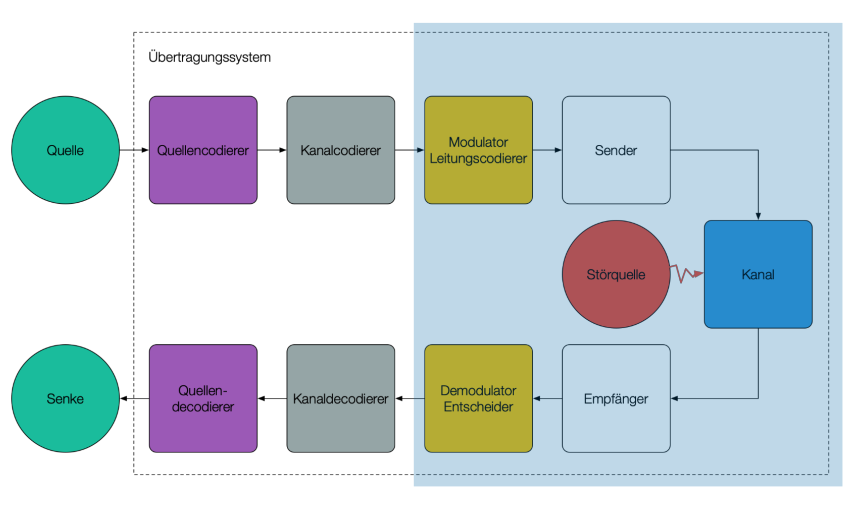
\includegraphics[width=.9\linewidth]{img/modell_der_informationsverarbeitung.png}
\caption{\label{fig:orgd3d37be}Model of information processing}
\end{figure}

\textbf{Probability}
TODO!

\textbf{Source and Sink}

Jeden Quelle hat ein Zeichenvorrat.
Nachricht wird kodiert und wird über Kanal übertragen.
Senke hat auch ein Zeichenvorrat und muss das übertragene Wort entscheiden und interpretieren.
Dafür müssen die Zeichenvorräte der Quelle und Senke übereinstimmen.

\begin{itemize}
\item Wenn Zeichenvorrat ungleich: information irrelevant
\item Wenn Zeichenvorrat:
\begin{itemize}
\item wort redundant: vorhersagbar
\item wort nicht redundant: \emph{Information}
\end{itemize}
\end{itemize}


\begin{figure}[htbp]
\centering
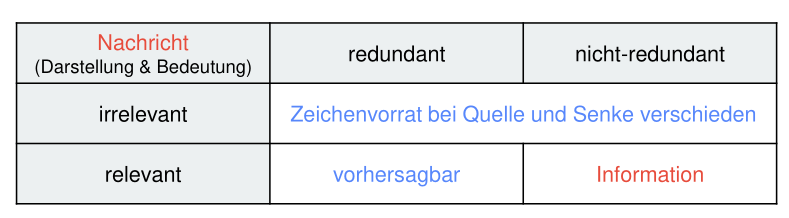
\includegraphics[width=.9\linewidth]{img/informations_uebertragung_information.png}
\caption{\label{fig:org3e104ad}Information, Nachricht}
\end{figure}

\textbf{Entscheidungsgehalt}

Mass für die minimale Anzahl Entscheidungen die getroffen werden müssen, um ein Zeichen zu erkennen.
Dies geschieht unter der Annahme dass alle Zeichen gleich Wahrscheinlich sind.
Dies kann in einem \href{../../../roam/20210806225200-binary_tree.org}{Binary Tree} abgebildet werden und entspricht der Höhe bzw. dem \(\log_2\) der Anzahl Blätter.

\begin{equation}
H_0 = \log_2(N)[bit]
\end{equation}

\begin{figure}[htbp]
\centering
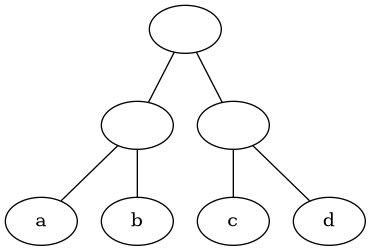
\includegraphics[width=.9\linewidth]{img/entscheidungsgehalt_tree.png}
\caption{\label{fig:org285df54}Entscheidungsgehalt}
\end{figure}

Zeichenvorrat: X = \{a, b, c, d\}, N = 4 verschieden Zeichen.
Daher ist der Informationsgehalt \(H_0 = \log_2(4) = 2\).
Das sieht man auch ihm Baum \ref{fig:org285df54}.
Es müssen zwei Entscheidungen getroffen werden, um zu einem Zeichen zu gelangen.

\textbf{Entscheidungsfluss}

Der Entscheidungsfluss ist der \href{../../../roam/20211001174136-was_ist_der_entscheidungsgehalt.org}{Entscheidungsgehalt} im Verhältnis zu der Übertragungszeit eines Quellenzeichens.

\begin{equation}
H_0^* = \frac{\log_2(N)}{\tau}[\frac{\text{bit}}{s}]
\end{equation}

\textbf{Informationsgehalt eines Zeichens}

Der Informationsgehalt eines Zeichens sagt aus, wie viele Entscheidungen zu treffen sind, um das zu Zeichen zu bestimmen.
Mit anderen Worten, wie viele mal muss ich zwischen Rechts / Links im Baum entscheiden, bis ich das Zeichen erreicht habe.

\begin{itemize}
\item \(p(x_k)\) entspricht der Auftrittswahrscheinlichkeit des Zeichen \(x_k\)
\end{itemize}

\begin{align}
I(x_k) &= \log_2(\frac{1}{p(x_k)}) [bit] \\
&= -\log_2(p(x_k)) [bit]
\end{align}

\textbf{Entropie}

Als Entropie bezeichnet man den mittleren \href{../../../roam/20211001175826-was_ist_der_informationsgehalt_eines_zeichen.org}{Informationsgehalt} einer Quelle.
Entropie beschreibt wie viele Entscheidungen die Qulle / Senke im Mittel pro Zeichen treffen muss.
Ist also nichts anderes als der Mittelwert über den \href{../../../roam/20211001175826-was_ist_der_informationsgehalt_eines_zeichen.org}{Informationsgehalt}.

\begin{itemize}
\item \(p(x_k)\): Die Wahrscheinlichkeit des Zeichen \(x_k\)
\item \(I(x_k)\): Der Informationsgehalt des Zeichen \(x_k\)
\end{itemize}

\begin{align}
H(X) &= \sum_{k=1}^N p(x_k) \cdot I(x_k) \\
&= \sum_{k=1}^N p(x_k) \cdot (-1)\log_2(p(x_k))
\end{align}

\textbf{Redundanz der Quelle}

Wenn die Auftrittswahrscheinlichkeit aller Zeichen gleich ist, ist der Informationsgehalt am grössten, bzw. die Redundanz am kleinsten.
Die Redundanz der Quelle ist die Differenz ziwchen \href{../../../roam/20211001174136-was_ist_der_entscheidungsgehalt.org}{Entscheidungsgehalt} und der \href{../../../roam/20211001180418-was_ist_die_entropie_in_der_informationstheorie.org}{Entropie}. 
\begin{itemize}
\item \(H_0\) ist der \href{../../../roam/20211001174136-was_ist_der_entscheidungsgehalt.org}{Entscheidungsgehalt}
\item \(H(X)\) ist die \href{../../../roam/20211001180418-was_ist_die_entropie_in_der_informationstheorie.org}{Entropie}
\end{itemize}


\begin{equation}
R_Q &= H_0 - H(X)
\end{equation}

\textbf{Kleinste Redundanz}

\emph{Annahme}: alle Zeichen sind gleich wahrscheinlich (a,b,c,d).
Dann würde sich ein Baum wie in \ref{fig:org16544c6} in aufspannen.
Dieser ist der selbe wie im \href{../../../roam/20211001174136-was_ist_der_entscheidungsgehalt.org}{Entscheidungsgehalt}.
Folglich wird \(R_Q = x - x = 0\) gerechnet.

\begin{figure}[htbp]
\centering
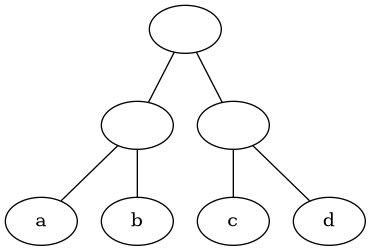
\includegraphics[width=.9\linewidth]{img/entropie_alle_gleich.png}
\caption{\label{fig:org16544c6}Tree mit gleichmässiger Auftrittswahrscheinlichkeit}
\end{figure}

\textbf{Codewortlänge}

Die tatsächlie Codewortlänge muss eine Ganzzahl sein, weil man keine Halbenbits übertragen kann.
Die Codewortänge für ein Zeichen lässt sich wie folgt berechnen:
\begin{itemize}
\item \(I(x_k)\) entspricht dem \href{../../../roam/20211001175826-was_ist_der_informationsgehalt_eines_zeichen.org}{Informationsgehalt}.
\end{itemize}

\begin{align}
L(x_k) &= \lceil I(x_k) \rceil \\
&= \lceil \log_2(\frac{1}{p(x_k)}) \rceil \\
&= \lceil -\log_2(p(x_k)) \rceil
\end{align}

\textbf{Entropie eines Codes}

Die Entropie des Codes entspricht dem Mittelwert der \href{../../../roam/20211001182658-warum_muss_die_codewortlange_eine_ganzzahl_sein.org}{Codewortlänge}:
\begin{itemize}
\item \(L(x_k)\) enspricht der \href{../../../roam/20211001182658-warum_muss_die_codewortlange_eine_ganzzahl_sein.org}{Codewortlänge}
\end{itemize}

\begin{align}
H_C(X) &= \sum_{k=1}^N p(x_k) \cdot L(x_k) [\frac{\text{bit}}{\text{Zeichen}}]
\end{align}

\textbf{Shannonsches Codierungstheorem}

Für jede beliebige Binärcodierung mit Präfixeigenschaft ist die \href{../../../roam/20211001191148-was_ist_die_entropie_eines_codes.org}{mittlere Codewortlänge} nicht kleiner als die \href{../../../roam/20211001180418-was_ist_die_entropie_in_der_informationstheorie.org}{Entropie}:

\begin{equation}
H(X) \leq L(X)
\end{equation}

Für jede beliebige Quelle kann eine Binärcodierung gefunden werden, so dass die folgende Ungleichung gilt:
\begin{equation}
H(X) \leq L(X) \leq H(X) + 1
\end{equation}

\textbf{Redundanz des Codes}

Redunanz des Codes:
\begin{itemize}
\item \(L(x_k)\) entspricht der Codewortlänge
\item \(H(X)\) entspricht der Entropie
\end{itemize}


\begin{equation}
R_C &= L - H(X)
\end{equation}

\textbf{Quelle ohne Gedächnis}

Bei einer Quelle ohne Gedächnis ist die Auftritswahrscheinlichkeit eines Zeichen unabhängig davon, welche Zeichen zuvor generiert wurde.
Die mittlere Entropie einer Quelle ohne Gedächtnis ist stets grösser oder gleich der Entropie einer Quelle mit Gedächtnis.

Die \href{../../../roam/20211002171445-verbundswahrscheinlichkeit.org}{Verbundswahrscheinlichkeit} ist für zwei Zeichen \(x_i\) und \(y_k\):
\begin{equation}
p(x_i, y_k) = p(x_i) \cdot p(y_k)
\end{equation}

\textbf{Gedächnisbehaftete Quelle}

Eine Quelle mit Gedächnis merkt sich, welches Zeichen bereits generiert wurde.
Dadurch ist dich \href{../../../roam/20211002171445-verbundswahrscheinlichkeit.org}{Verbundswahrscheinlichkeit} wie folgt definiert:


\begin{equation}
p(x_i, y_k) = p(x_i) \cdot p(y_k)
\end{equation}

Die Verbundsentropie ist wie folgt:
\begin{equation}
H(X, Y) = H(X) + H(X|Y)
\end{equation}

Die mittlere Entropie einer Quelle ohne Gedächtnis ist stets grösser oder gleich der Entropie einer Quelle mit Gedächtnis.

\textbf{Verbundsentropie}

\begin{align}
H(X,Y) &= \sum_{i=1}^N \sum_{k=1}^N p(x_i, y_k) \cdot -\log_2(p(x_i,y_k))
\end{align}

\begin{equation}
H(X,Y) = H(X) - H(Y|X)
\end{equation}

\textbf{Präfixfreier Code}

\begin{quote}
Kein Codewort des Codes ist Präfix eines anderen Codewortes.
Anders ausgedrückt darf kein Codewort den Beginn eines anderen Codewortes darstellen.
Ein Code zum Beispiel mit den Codewörtern \{0, 10, 11\} erfüllt die Präfix-Eigenschaft, während hingegen der Code mit den Codewörtern \{0, 01, 10\} sie nicht erfüllt, da „0“ Präfix von „01“ ist.

-- Wikipedia, 2022
\end{quote}


\textbf{Typen Source Encoder}

In the \href{../../../roam/20211001174201-information_theory.org}{information theory} exists two types
\begin{itemize}
\item data compressor
\begin{itemize}
\item lossless (verlustfrei)
\item lossy (verlustbehaftet)
\end{itemize}
\item encryption
\begin{itemize}
\item symmetric
\item asymmetric
\end{itemize}
\end{itemize}

\textbf{Verlustfreie Kompression}

The goal of a compression is make the data transfer and storing as efficient as possible. This is achieved with reducing the redundancy and remove not used elements.

A good compression algorithm has a:
\begin{itemize}
\item high encode / decode speed
\item low requirements for hardware
\end{itemize}


There exists two kind of lossless compression:
\begin{itemize}
\item static procedure (adaptive): character of the data used
\item dynamic procedure: character of the data is \textbf{not} used. In a worst case scenario the data are bigger with compression
\end{itemize}


\textbf{Huffman Code}

Procedure:
\begin{enumerate}
\item sort the symbols after possibility of occurrence
\item repeat
\begin{enumerate}
\item sum up the possibilities of the two least possible symbols
\item the less possible symbol got the 1 the other the 0
\item this two counts now as one symbol
\item repeat this until only every symbols is processed
\end{enumerate}
\end{enumerate}


\begin{figure}[htbp]
\centering
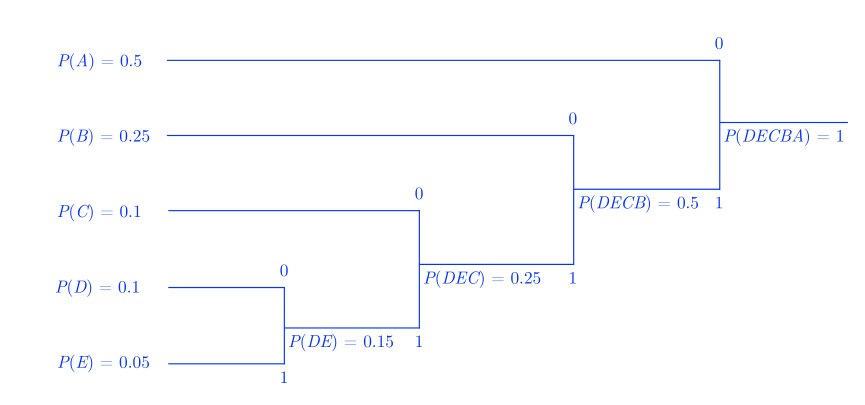
\includegraphics[width=.9\linewidth]{img/hufman.png}
\caption{\label{fig:org7f196c3}Hufman Example}
\end{figure}

\textbf{Lauflängenkodierung}

The Run Length Encoding RLE (de. Lauflängenkodierung) is a \href{../../../roam/20211014093202-lossless_compression.org}{Lossless compression}.
If a symbol occurs more than one in a row then the number of repetition is prefix with the character appended. 

\begin{verbatim}
Quelltext w: Agggbbehfffgggg => |w| = 15
Codiert w_c: A3g2beh4f5g => |w_c| = 11
\end{verbatim}

This compression is very interesting for binary because the transmission is always just a repetition of 0 and 1.
First both parts has to agree with witch number the transfer starts.
After that only the number of 0 or 1 is transmitted

\begin{verbatim}
0000 0111 => 5 3
\end{verbatim}

\textbf{Lempel-Ziv Algorithmus}

During the encoding (runtime) a code book is created on the fly.
If a pattern is already transmitted only the reference to this pattern is transmitted.


Der zu komprimierende Code hat wiederkehrende Mustr oder PHrasen, nur die codierten Phrasen müssen übertragen werden.
Währende des Durchlaufens der Daten wird ein ständig wachsender Baum erzeugt.
Baum dient als Wörterbuch.
Knoten dienen als Referenz.


The algorithms needs:
\begin{itemize}
\item a search buffer (the already encoded symbols)
\item a look-ahead buffer (shows the next symbols to encode)
\item if a sequence of symbols in the look-ahead buffer and the search buffer are equal
\begin{itemize}
\item then a code consisting of position and length and stored
\item else the code is stored as in the look-ahead buffer.
\end{itemize}
\end{itemize}


\begin{figure}[htbp]
\centering
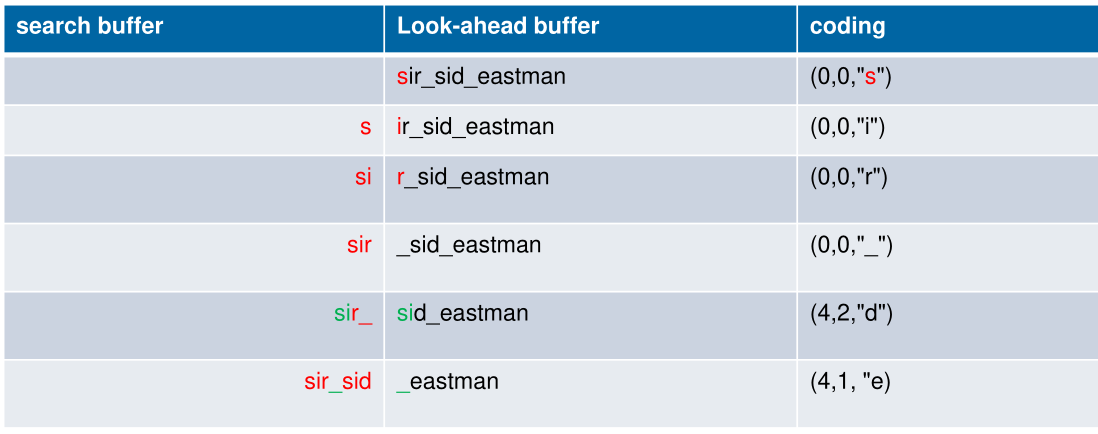
\includegraphics[width=.9\linewidth]{img/lempel_ziv_example.png}
\caption{\label{fig:orgec1b335}Lempel-Ziv Example}
\end{figure}

\textbf{Transposition Cipher}

In a transposition cipher every symbol stays the same (no substitution used).
Only the order of the symbols is changed.
A simple example is shown below:

The clear text "Hello my World" is inserted in a table by row:

\begin{center}
\begin{tabular}{llll}
H & E & L & L\\
O & M & Y & W\\
O & R & L & D\\
\end{tabular}
\end{center}

and now read the text by column: HOOEMRLYLLWD

\textbf{DES}

DES is a symmetric key algorithm and was long the standard for data encryption.
Today it is not safe anymore because of its short key length (max. 56 bits) and therefore should not be used anymore.

\textbf{Inverse einer Zahl}

In math a number \(x\) is called the inverse of \(y\) when \(x \cdot y = 1\).
In general this is the case when \(y = x^{-1}\).
Interesting is when modulo is used.
Because now you can multiple \(a\) with \(b \ne a^{-1}\) to get -1

\begin{equation}
a \cdot b \mod c \equiv 1
\end{equation}

\textbf{Euler Function}

The Euler function returns for a given \(n\) the amount of part-unrelated (de: teilerfremd) numbers \(n\).
The symbol for the Euler function is \(\Phi\)

The Euler function is difficult to calculate except for prime numbers:
Be \(n\) a prime number
\begin{align}
\Phi(n) = n - 1
\Phi(5) = 5 - 1 = 4
\end{align}

The result of \(\phi(p \cdot q)\) where \(p\) and \(q\) are prime is:
\begin{align}
\Phi(p \cdot q) &= \Phi(p) \cdot \Phi(q) \\
&= (p - 1) \cdot (q - 1)
\end{align}

\textbf{Euler Theorem}

For two part-unrelated numbers \(a < b\) applies the following:
\begin{equation}
a^{\Phi(b)} \mod b \equiv 1
\end{equation}


\(\Phi(b)\) is called Eulers funciton.

\textbf{Euler Function \& Theorem}

If you combine Euler's Function with his theorem you can say something like this:
If \(b = p \cdot q\) where p and q are prime then:
\begin{align}
a^{\Phi(b)} \mod b \equiv & \\
a^{\Phi(p \cdot q} \mod (p \cdot q) \equiv & \\
a^{(p - 1) \cdot (q-1)} \mod (p \cdot q) \equiv & 1
\end{align}

\textbf{RSA Parameters}

\begin{enumerate}
\item Choose \(p\) and \(q\)
\begin{enumerate}
\item \(n = p_1 \cdot p_2\)
\item \(n\) is public, \(p\), \(q\) private
\end{enumerate}
\item Calculate \(\Phi(n)\)
\item Choose \(e\)
\begin{itemize}
\item \(e\) has to be part-unrelated to \(\Phi(n)\) and \(1 < e < \Phi(n)\)
\item in reality often 3 or 65537
\end{itemize}
\item Calculate the inverse from \(e\) resulting in \(d\)
\begin{itemize}
\item For Example with the \href{../../../roam/20211104174408-extended_euclidean_algorithm.org}{Extended Euclidean algorithm}
\end{itemize}
\end{enumerate}


Be \(m\) the message. Then to encrypt: \(c = m^e \mod n\).
Do decrypt \(c\) to \(m\): \(m = c^d \mod n\).

\begin{figure}[htbp]
\centering
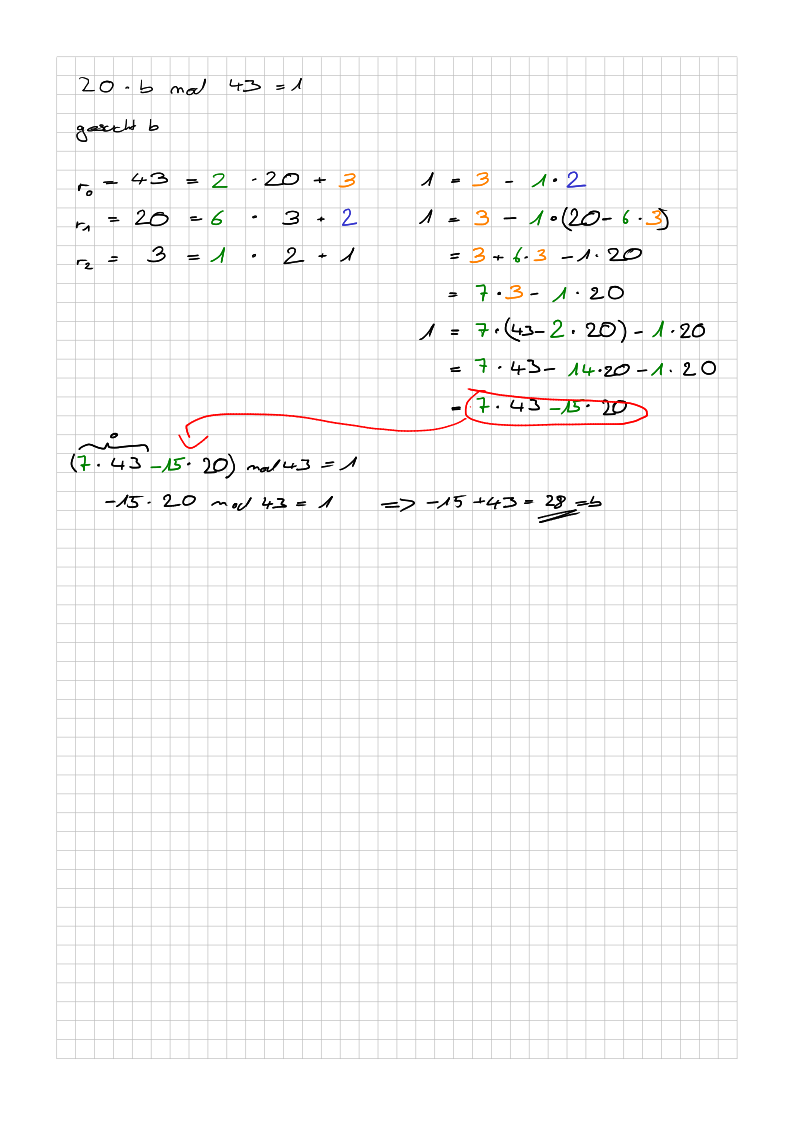
\includegraphics[width=.9\linewidth]{img/rsa_nach_rinkel.png}
\caption{\label{fig:org4a759ac}RSA nach Rinkel}
\end{figure}

\textbf{Channel Matrix}

Die Kanalmatrix beschreibt wie Wahrscheinlich es ist, dass man \(y\) erhält, wenn \(x\) gesendet wurde.
\(p\) und \(q\) geben an, wie wahrscheinlich es ist, dass ein Fehler auftritt.

\begin{align}
  p(Y|X) =
  \begin{bmatrix}
    \sum = 1 \\
    \sum = 1
  \end{bmatrix}
=
  \begin{bmatrix}
    p & 1 - p \\
    1 - q & q \\
  \end{bmatrix}
=
  \begin{bmatrix}
    p(y_1|x_1) & \cdots & p(y_n|x_1) \\
    \vdots & \ddots & \vdots \\
    p(y_1|x_m) & \cdots & p(y_n|x_m) \\
  \end{bmatrix}
\end{align}

\begin{align}
  \begin{bmatrix}
    p(y_1) \\
    p(y_2)
  \end{bmatrix}
  = 
  \begin{bmatrix}
    p(x_1) \cdot p(y_1 | x_1) + p(x_2) \cdot p(y_1|x_2) \\
    p(x_1) \cdot p(y_2 | x_1) + p(x_2) \cdot p(y_2|x_2)
  \end{bmatrix}
\end{align}

\begin{figure}[htbp]
\centering
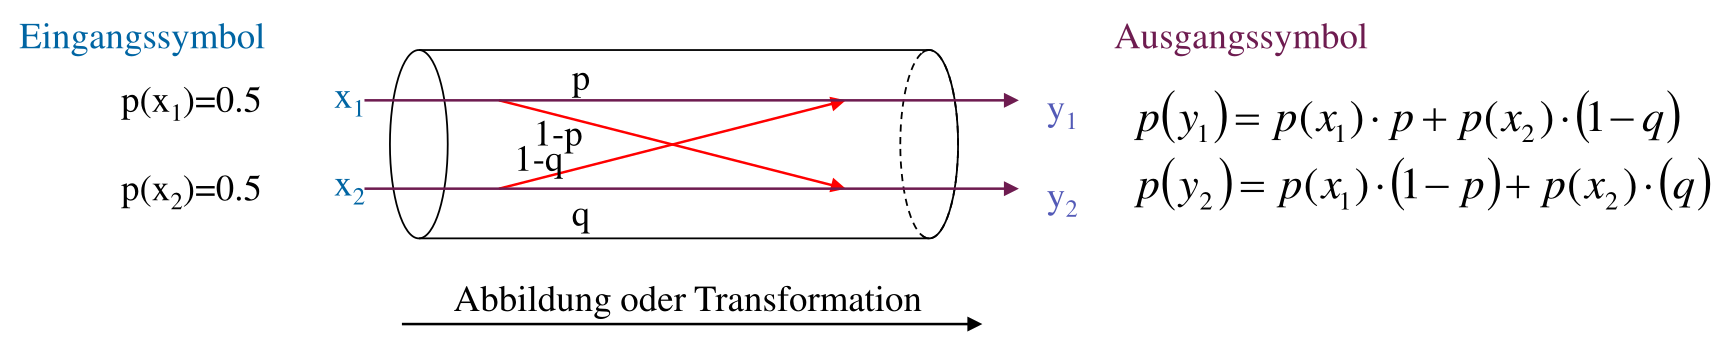
\includegraphics[width=.9\linewidth]{img/kanalmatrix_modell.png}
\caption{\label{fig:orgc789d1a}Channel Matrix Model}
\end{figure}

\textbf{Maximum Likelihood}

How high is the possibility that I receive \(y_1\) when \(x_1\) is sent.
The cell with the highest value in a column (y-value) is maximum likelihood the x-value which was sent.

\begin{equation}
\label{eq:org982e49b}
  p(Y|X) =
  \begin{bmatrix}
    0.6 & 0.2 & 0.2 \\
    0.2 & 0.2 & 0.6 \\
    0.3 & 0.2 & 0.5 \\
  \end{bmatrix}
\end{equation}

When I got a \(y_1\) (first column in \ref{eq:org982e49b}) then it probably \(x_1\) was sent.
When I got a \(y_3\) then probably a \(x_2\) was sent.
And to cover all possible \(x\) values the \(y_2\) is mapped to \(x_2\).

\textbf{Mutual Information / Transinformation}

Mutual information describes how much two random variables correlate.
The higher the more they correlate (1 total correlation, 0 no correlation).

In the context of information transfer over a channel the mutual information describes also how big the flow is which I can transfer without errors.
Transiformation (T) ist der Informationsfluss, den ich fehlerfrei über einen gestörten Kanal übertragen kann.

\begin{figure}[htbp]
\centering
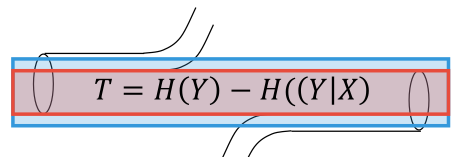
\includegraphics[width=.9\linewidth]{img/transinformation.png}
\caption{\label{fig:org459a31b}Transinformation / Mutual Information}
\end{figure}


\begin{align}
  H(Y|X) &= -\sum_i^n\sum_j^n p(x_i)\cdot p(y_j|x_i) \cdot \log_2(p(y_j|x_i)) \\
  T &= H(Y) - H(Y|X) = H(X) - H(X|Y)
\end{align}

\textbf{Wie ändert die Kanalmatrix die Transinformation}

Ein nicht gestörter Kanal (Einheitsmatrix) überträgt den mittleren Informationsgehalt.
Transinformation wird nur durch die Quelle bestimmt.
Verändert sich die Entropie der Quelle, ändert sich die Transinformation.
Nimmt die Fehlerwahrscheinlichkeit zu, nimmt die Transinformation ab.
Sind in der Kanalmatrix alle Positionen gleich besetzt, wird die Transinformation \(T = 0\).

\textbf{Coderaum}

The Code space is a set of code words / code points.

\textbf{Hamming Distance}

When one code word is given the Hamming Distance (\(h\)) describes how many positions have to change until a new valid code word is reached.

\begin{itemize}
\item Number of reliable detectable errors (\ref{eqn:detectableErrors})
\item Number of reliable correctable errors (\ref{eqn:correctableErrors})
\end{itemize}

\begin{align} 
  e^* &= h - 1 \label{eqn:detectableErrors} \\
  e &= 
  \begin{cases}
    \frac{h-2}{2} & \mbox {if h is even} \\
    \frac{h-1}{2} & \mbox {if h is odd}
  \end{cases} \label{eqn:correctableErrors}
\end{align}

\textbf{Korrigierkugel}

The correction sphere has a radius of \(e\): the number of reliable correctable errors.
The center of a correction sphere is always a \emph{valid} code word.
If you receive a invalid code word and this code word is inside of the sphere then it will be changed to the center / valid code word.

\begin{figure}[htbp]
\centering
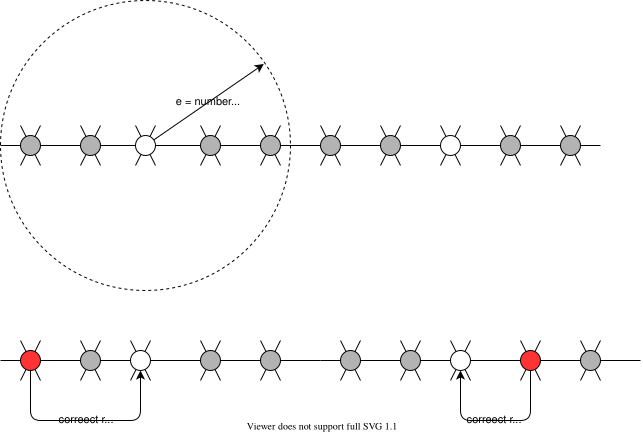
\includegraphics[width=.9\linewidth]{img/hamming_korrigierkugel.drawio.png}
\caption{\label{fig:org843424a}Korrigierkugel / Correction Sphere}
\end{figure}

\textbf{Perfecter Code / Dichtgepackter Code}

A code space is called a perfect code when every code word (valid or invalid) is in a correction circle.

\begin{itemize}
\item \emph{n}: The dimension of the code (number of all code words (CW) = \(2^n\))
\item \emph{m}: The dimension of message (number of all valid CW = \(2^m\))
\item \emph{k}: The dimension of check positions (\(n=m+k\))
\end{itemize}

Then applies:
\begin{equation}
  2^m \cdot \sum_{w=0}^e \begin{pmatrix} n \\ w \end{pmatrix} \leq 2^n
\end{equation}

\begin{itemize}
\item \emph{2\textsuperscript{m}}: Number of valid CW (or number correction circles)
\item \emph{\(\sum\)}: Number of CW per correction circle
\item \emph{2\textsuperscript{n}}: Number of all CW
\end{itemize}

In the following case we call the code perfect:
\begin{equation}
  2^m \cdot \sum_{w=0}^e \begin{pmatrix} n \\ w \end{pmatrix} = 2^n
\end{equation}

\textbf{Haming Codes}

Hamming Code is a family of error correcting codes.
Every Hamming Codes has a Haming Distance of 3.


Hamming Codes can be built with either a generator matrix or with a Generator Polynom.

\textbf{Generator Matrix Hamming Code}

The generator matrix consists of two parts.
The first indicates witch you need to pick for you calculation (this with 1).
And the second part is the unit matrix which marks the control positions.

A generator matrix has two conditions:
\begin{enumerate}
\item every vector of the message part has to be different than the others
\item the equation \ref{eqn:matrixCondition} has to be fullfield
\end{enumerate}

\begin{equation}\label{eqn:matrixCondition}
  \sum_i x_i \cdot \vec{P_i} \equiv \vec{0} \mod 2
\end{equation}


An example of valid generator matrix is shown in \ref{eqn:matrixExample}
\begin{equation}\label{eqn:matrixExample}
  \left[
    \begin{array}{cccc|ccc}
      1 & 1 & 1 & 0 & 1 & 0 & 0 \\
      0 & 1 & 1 & 0 & 0 & 1 & 0 \\
      1 & 1 & 0 & 1 & 0 & 0 & 1 \\
    \end{array}
    \right]
\end{equation}

If only one bit is changed during transmission then the calculation of \ref{eqn:matrixCondition} is wrong.
The result is the vector which has changed.

\textbf{Generator Polynom Hamming Code}

The generator matrix can be replaced with a polynom.
This has the benefits that it is easier to calculate the control positions.

\begin{itemize}
\item \emph{k}: Number of control positions
\item \emph{n}: Dimension of the code
\end{itemize}

Where \(g_i={0,1}\)
\begin{align}
  G(u) = \sum_{i=0}^k g_i\cdot u^i \label{eqn:generatorPolynom} \\
  X(u) = \sum_{i=0}^n g_i\cdot u^i \label{eqn:codeWordPolynom}
\end{align}

If the code word polynom (\ref{eqn:codeWordPolynom}) can be divided by the generator polynom (\ref{eqn:generatorPolynom}) mod 2 it is a valid code:

\begin{align}
  Q(u) &= X(u) / G(u) \\
  X(u) / G(u) &\equiv Q(u) \mod 2 \equiv 0
\end{align}

\begin{figure}[htbp]
\centering
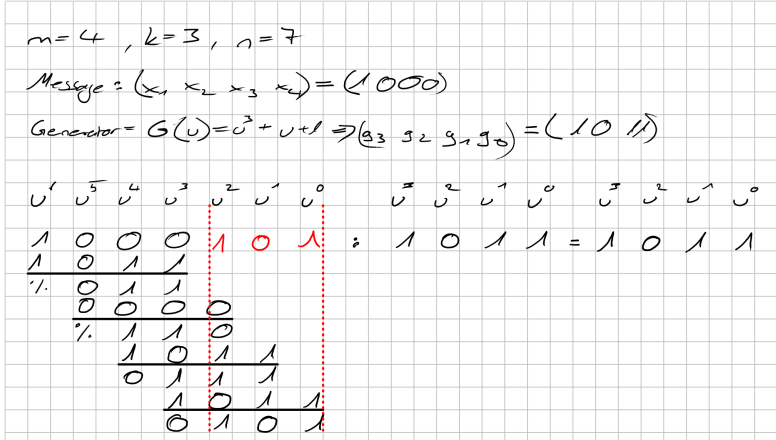
\includegraphics[width=.9\linewidth]{img/polynom_generator.png}
\caption{\label{fig:orgb3c478c}Generator Polynom Hamming Code}
\end{figure}

To verify if received message is correct divide the message through the generator polynom. If this is not 0 then an error is occurred.
\begin{equation}
  \begin{cases}
    \mbox{No errors} & \mbox{if Message} / G(u) = 0 \\
    \mbox{Errors(s) occurred} & \mbox{if Message} / G(u) \ne 0
  \end{cases}
\end{equation}

\textbf{Was ist ein Blockcode}

Your data is grouped in blocks and then each block is encoded seperately.
Block codes are easy to implement and have a hight error detection.
But you have to build blocks.
Therefore, streams are not possible to encode.

\textbf{Faltungscodes / Convolutional Codes}

With Convolutional codes streaming data (code block length not known) can be encoded.
This kind of code is often used in the mobile network.
Convolutional codes do not need any block synchronization.

\textbf{How does Convolutional Codes work}

A Convolutional codes has storage cells for the previous send bits.
The highets bits in the generator polynom tells you how many Storage Cells you have.
The bit from the past is \emph{xor-ed} with the current one.

In the figure \ref{fig:org89ff4c4}  the upper way is the \(g_1\) and the lower \(g_2\).
If a bit was used it shift one further to the storage cell.

\href{../../../roam/20211105145648-the_generator_polynom_for_hamming_codes.org}{The Generator Polynom} can be read from the diagram:
\begin{itemize}
\item \(g_1(x) = 1 + x^2\): The upper way
\item \(g_2(x) = 1 + x + x^2\): The bottom way
\end{itemize}


The number of tails bits are the same as the number of storage cells.
The encoder in figure \ref{fig:org89ff4c4} has two storage cells.
Therefore two tailbits are needed.


\begin{table}[htbp]
\caption{\label{tab:org1be964a}Output for input 100}
\centering
\begin{tabular}{rrrr}
\(x_i\) & \(g_1(x_i)\) & \(g_2(x_i)\) & output\\
\hline
1 & 1 & 1 & 11\\
0 & 0 & 1 & 01\\
0 & 1 & 1 & 11\\
0 & 0 & 0 & 00\\
0 & 0 & 0 & 00\\
\end{tabular}
\end{table}

\begin{figure}[htbp]
\centering
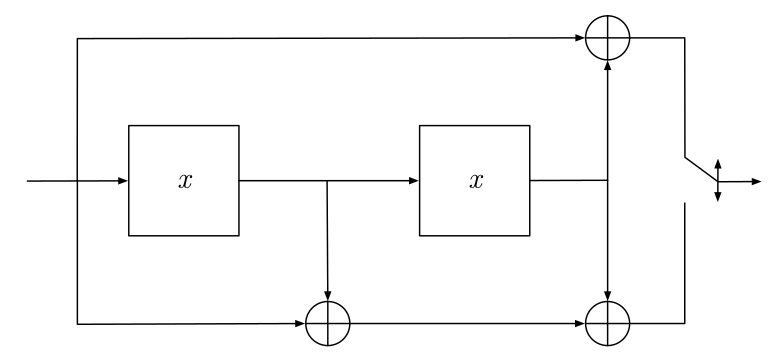
\includegraphics[width=.9\linewidth]{img/encoders_faltungscodes.png}
\caption{\label{fig:org89ff4c4}Faltungscode Encoder}
\end{figure}


\textbf{State Machine for Convolutional Codes}

A Convolutional Code can also be represented as a \href{../../../roam/20211108155646-state_machine_diagram.org}{State Machine Diagram}.
For an example see figure \ref{fig:org0766b1b}.
\href{../../../roam/20211105145648-the_generator_polynom_for_hamming_codes.org}{The Generator Polynom} \(g_1(x)\) and \(g_2(x)\) are as follows:

\begin{itemize}
\item \(g_1(x) = 1 + x^2\)
\item \(g_2(x) = 1 + x + x^2\)
\end{itemize}


\begin{enumerate}
\item Find the numbers of Storage cells \(n\)
\item Calculate the number of state \(m = 2^n\)
\item Build the table (\ref{tab:org5c9f7f2})
\item Build from table the \href{../../../roam/20211108155646-state_machine_diagram.org}{State Machine Diagram} / \href{../../../roam/20211109182310-deterministic_finite_automaton.org}{DFA}
\end{enumerate}


\begin{table}[htbp]
\caption{\label{tab:org5c9f7f2}Table of States for Code}
\centering
\begin{tabular}{lrlll}
State & Input & Cells & Output & Next State\\
\(S_0\) & 0 & 0 0 & 0 0 & \(S_0\)\\
\(S_0\) & 1 & 0 0 & 1 1 & \(S_2\)\\
\(S_1\) & 0 & 0 1 & 1 1 & \(S_0\)\\
\(S_1\) & 1 & 0 1 & 0 0 & \(S_2\)\\
\(S_2\) & 0 & 1 0 & 0 1 & \(S_1\)\\
\(S_2\) & 1 & 1 0 & 1 0 & \(S_3\)\\
\(S_3\) & 0 & 1 1 & 1 0 & \(S_1\)\\
\(S_3\) & 1 & 1 1 & 0 1 & \(S_3\)\\
\end{tabular}
\end{table}


\begin{figure}[htbp]
\centering
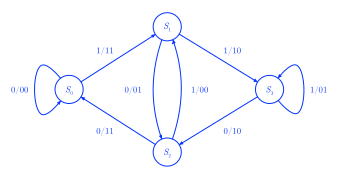
\includegraphics[width=.9\linewidth]{img/faltungscodes_state_machine_diagram.png}
\caption{\label{fig:org0766b1b}Convolutional Code as State Machine Diagram}
\end{figure}

\textbf{Trellis Diagram}

To visualize how the convolutional code is encoded over time the trellis diagram is suitable.
Each state of the state machine is only used once per CPU clock.
And the transition goes to the next state in the next CPU clock.


\begin{figure}[htbp]
\centering
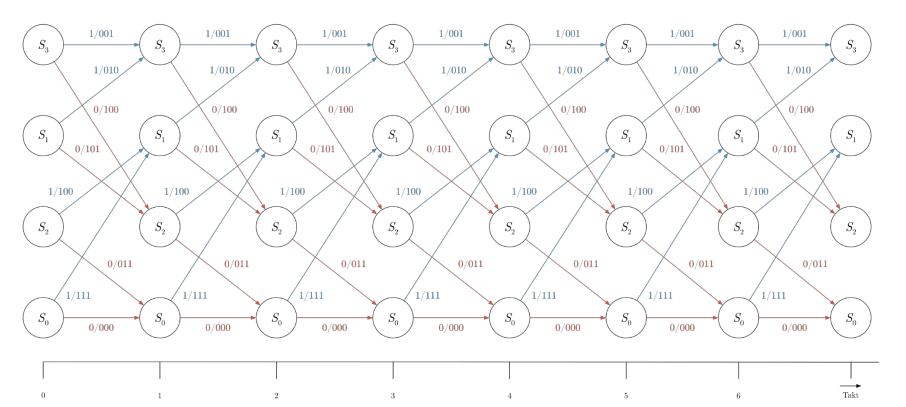
\includegraphics[width=.9\linewidth]{img/trellisdiagramm.png}
\caption{\label{fig:org99c4bcf}Trellis diagram}
\end{figure}

\textbf{Decode Convolutional Codes}

To decode a Convolutional Code you try to find the cheapest way throug the trellis diagram.
You start at the Starting State (\(S_0\)).
You compare each code word part with the possible transitions.
The transition which needs the fewest changes is used.


\begin{figure}[htbp]
\centering
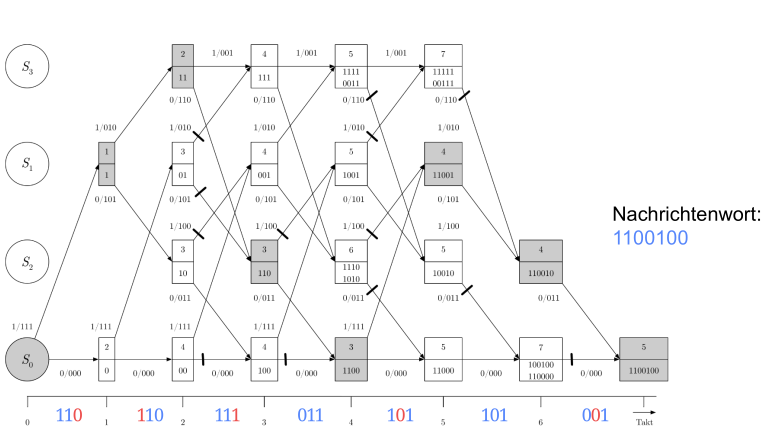
\includegraphics[width=.9\linewidth]{img/decode_convoluitonal_code.png}
\caption{\label{fig:orgb6f6e18}Decoding a Convolutional Code}
\end{figure}

\textbf{Block Code Rate}

\begin{itemize}
\item \emph{m}: Encoding Storage
\item \emph{R}: Block code rate
\item \emph{x}: Encoded Bits
\end{itemize}

\begin{align}
  R &= \frac{encodeded bits}{sent bits} \\
  &= \frac{x}{2 \cdot (x + m)} \label{eqn:Block Code Rate}
\end{align}

In \ref{eqn:Block Code Rate} the 2 is needed because for each input bit two output bits are generated.
The \(m\) is required because you need to send \(m\) tail bits to clear the storage. 

\textbf{Impulse Response}

The Impulse Response is the output of a system (for example an encoder) with a brief input signal.
In numbers this would be 1000\ldots{}

\textbf{Detect Number of Storage Cells}

Using a Impulse Response you can detect how many storage cells are used in the convolutional code.
The 1 which is send must be cleared from all storage cells.
Therefore, the same number of 0 are sent as storage cells.

\textbf{Was ist das Basisband}

Baseband is the range of frequencies occupied by a signal that has not been modulated to other frequencies.
The frequency is unchanged.

\textbf{Line Coding}
TODO!!

\textbf{Requirements Line Coding}

\begin{itemize}
\item Synchronisation of the clock / phase at the receiver
After a long period of 1 you have to known how many 1 are sent
\item Avoiding direct current components (Gleichstromkomponenten)
\item Resistance to interference
\end{itemize}


\textbf{Classification Line Coding}

Line codes can be classified using two properties:
\begin{enumerate}
\item polarity (0 to u / -u to u)
\item impuls form (Return to Zero / No Return to Zero)
\end{enumerate}


\begin{figure}[htbp]
\centering
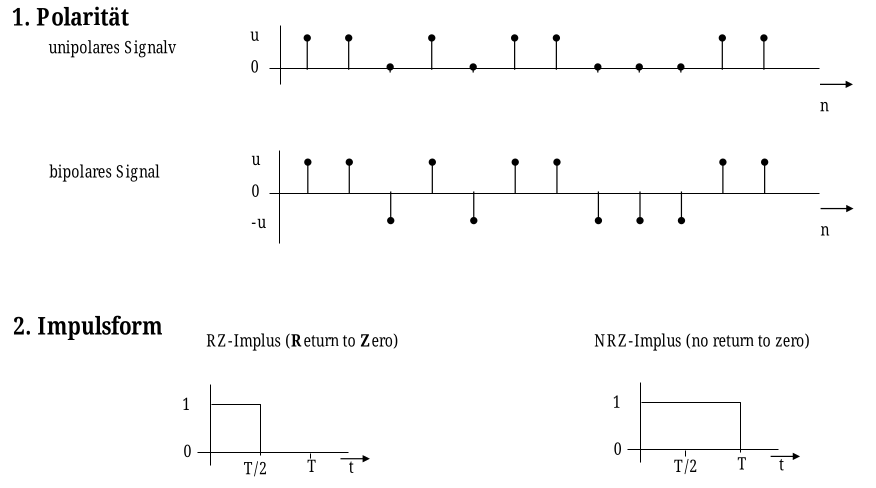
\includegraphics[width=.9\linewidth]{img/line_code_classification.png}
\caption{Line Code Classification}
\end{figure}

\textbf{Manchester Code}

The Manchester Code (see figure \ref{fig:org94325af}) has no direct current (Gleichstrom) but requireds the double amount of bandwith.
The Manchester Code by IEEE has the following convention:
\begin{itemize}
\item the 0 is represented as a high-low signal sequence
\item the 1 is represented as a low-high signal sequence
\end{itemize}


\begin{figure}[htbp]
\centering
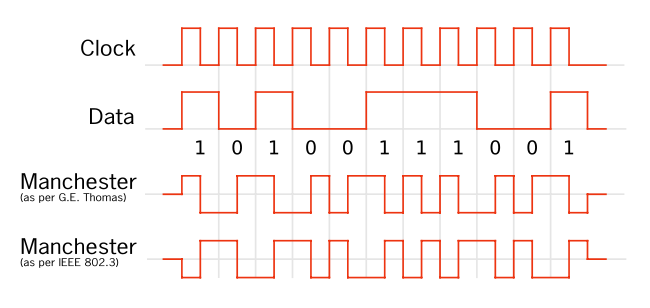
\includegraphics[width=.9\linewidth]{img/manchester_code.png}
\caption{\label{fig:org94325af}Machester Code}
\end{figure}

\textbf{AMI Code}

The AMI Code uses the following convention:
\begin{itemize}
\item the 0 is represented as a 0 level
\item the 1 is represented as an alternating level change of pos. and neg.
\end{itemize}


After a long sequence of 0 it is difficult for the receiver to know how many zeros actually were send.

\textbf{Parameter of a signal}

A signal consists of two parameters:
\begin{enumerate}
\item amplitude
\item period length / frequency (\href{../../../roam/20220101131242-period_length_vs_frequency.org}{Period Length vs. Frequency})
\end{enumerate}


\begin{figure}[htbp]
\centering
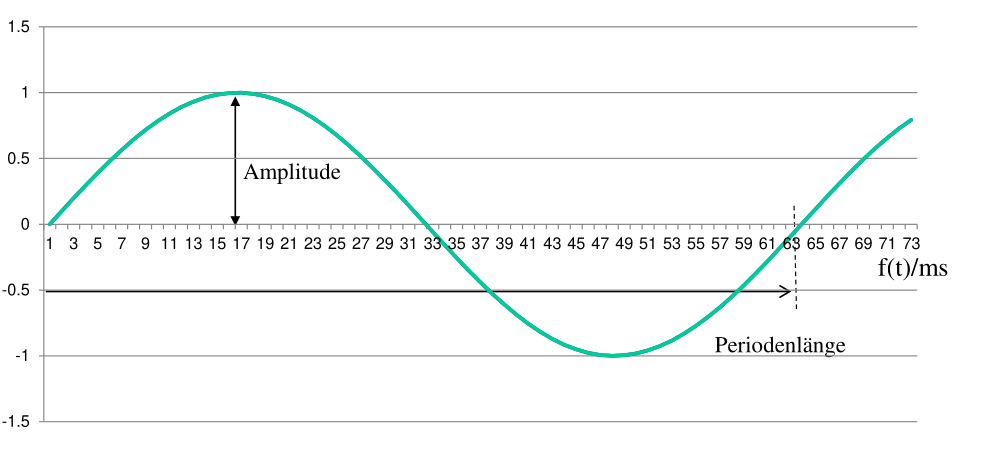
\includegraphics[width=.9\linewidth]{img/parameters_of_a_signal.png}
\caption{A Signal}
\end{figure}


\textbf{What are dB?}

Bel describes the ratio between two values.
For example the strength of an output and input signal.

\begin{equation}
S_{Bel} = \log_{10}(\frac{S_{out}}{S_{in}})
\end{equation}

The dezibel is more common than bel.

\begin{equation}
S_{dezibel} = 10 \cdot \log_{10}(\frac{S_{out}}{S_{in}})
\end{equation}

\emph{Example}
\begin{equation}
s_2 = 20,\, s_1 = 10
\end{equation}

\begin{align}
&  \log_{10}(\frac{s_2}{s_1}) \\
&= \log_{10}(\frac{20}{10}) \\
&= 0.301Bel \approx 3 dB
\end{align}

\textbf{Harmonische Schwingungen / Harmonic Oscillations}

Harmonic Oscillations are oscillations which does not have any sudden changes.
For example sine / cosine are harmonic.

In our world, all things consist of sine and cosine waves.
\end{document}